\def \Subject {Trees Game}
\def \Author {محمد امین قسوری}
\def \Date {1399/7/30}
\def \Session {9}
\setcounter{chapter}{\Session-1}

\chapter{\Subject}
\chapterauthor{\Author~ - \Date}

جزوه جلسه
\Session ام
 مورخ 
\Date
درس 
\CourseName
}
  تهیه شده توسط  
 \Author.
در جهت مستند کردن مطالب درس 
\CourseName

\section{مقدمه}
در این قسمت می خواهیم درمورد الگوریتم هایی صحبت کنیم که در بازی هایی که Single-agent نیستند و یک رقیب در مقابل خود داریم که گاها هوشمند و در بعضی مواقع نیز ممکن است اشتباه کند.

\section{تاریخچه ی بازی ها}
بعضی بازی ها مانند checkers حل شده (solved) هستند وحل شده به این معنی است که اگر هر دو بازیکن به صورت بهینه بازی کنند شما می توانید یک برد یا حداقل مساوی را بصورت قطعی بدست بیاورید (نبازید). از طرفی در مورد بعضی بازی ها مانند شطرنج نمی توان گفت که حل شده هستند.

\section{دسته بندی بازی ها}
تا به حال بازی‌ های زیادی انجام داده ایم. در این جا میخواهیم آن‎ها را بر اساس ویژگی هایی دسته بندی نماییم.

\subsection{Deterministic or Stochastic}
به بازی هایی که شانس در آن‎ها معیار نباشد،  deterministic  می گویند مانند GO یا شطرنج و به بازی هایی که با شانس همراه باشند Stochastic گفته می‎شود مانند تخته نرد که دو تاس درآن داریم و حرکات و تصمیمات بعدی ما به آن وابسته است.

\subsection{تعداد بازیکن ها}
تعداد بازیکن ها نیز معیاری برای دسته ‎بندی بازی ها هستند که بعضی مانند شطرنج دونفره و بعضی دیگر میتوانند چندین نفره باشند مانند خیلی از Game Board ها.

\subsection{Sum Zero}
این ویژگی نشان میدهد که آیا بازیکن ها کاملا بر خلاف و مقابل هم بازی میکنند یا خیر. برای مثال اگر هر دو یک هدف مانند برداشتن یک الماس داشته باشند خوب قطعا بر خلاف هم هستند و الماس را یکی از آن ها بدست می آورد و دیگری از دست میدهد.

\begin{figure}[h!]
    \centering
    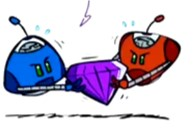
\includegraphics[width=0.3\linewidth]{images/zerosum.jpg}
    \caption{sum Zero}
\end{figure}


\subsection{Information Perfect}
یعنی درمورد بازی تمام اطلاعات و مواردی که برای تصمیم گیری لازم داریم در اختیار داریم.


در قسمت قبل از planning regular استفاده می کردیم منتهی در این جا پارامتری داریم که بر خلاف ما عمل میکند و ما نمی توانیم تمام تصمیمات خود را برنامه ریزی کنیم پس در ادامه از تعدادی الگوریتم برای محاسبه استراتژی بازی کردن در مقابل حریف صحبت خواهیم کرد.



\section{Games Deterministic}
ما میتوانیم بازی های deterministic به صورت زیر نمایش بدهیم.
\begin{itemize}
    \item
States هر وضعیت بازی یک حالت است مانند حالت اولیه.
    \item
Players همان بازیکن ها هستند.
    \item
Actions تصمیماتی که میتواینم در یک حالت بگیریم که می‎تواند وابسته به حالت یا بازیکن باشد. 
    \item
Function Transition خیلی مشابه function successor در search regular است.
    \item
Test Terminal تست می‎کند که آیا بازی تمام شده است یا خیر.
    \item
 Utilities Terminal همه ی نتیجه ها امتیازدهی می‎شوند و میتواند بجای سه مقدار بردن، باختن یا مساوی بازه ای از اعداد برای امتیازدهی داشته باشند.
 \end{itemize}


\section{Tree Agent Single}

\begin{figure}[h!]
    \centering
    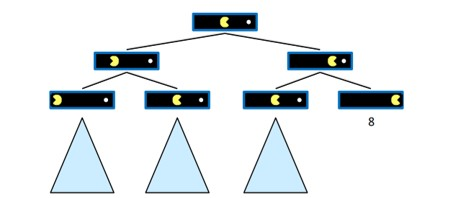
\includegraphics[width=0.8\linewidth]{images/singleagenttree.jpg}
    \caption{Tree Agent Single}
\end{figure}

برای pacman زمانی که یک agent داشته باشیم این درخت خیلی ساده است. ما مقداری از آن درخت را میکشیم و با توجه به این که با گذشت زمان امتیاز منفی خواهیم گرفت همه ی موارد سمت چپ کمتر از 8 خواهند شد و ما برای هر گره امتیازی در نظر میگیریم که در حقیقت ماکسیمم امتیازهای بچه هایش است.


\section{Search Adversarial}

\begin{figure}[h!]
    \centering
    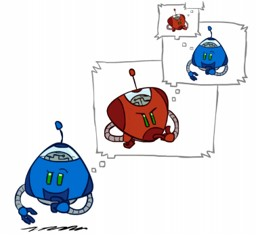
\includegraphics[width=0.6\linewidth]{images/adversarial01.jpg}
    \caption{Search Adversarial}
\end{figure}

در search adversarial بدلیل داشتن رقیب در بازی  باید به همه ی حالات فکر کنیم و تا چندین سطح به این فکر کنید که اگر چه حرکتی را بروید در نهایت امتیاز به نفع شما خواهد بود.

\begin{figure}[h!]
    \centering
    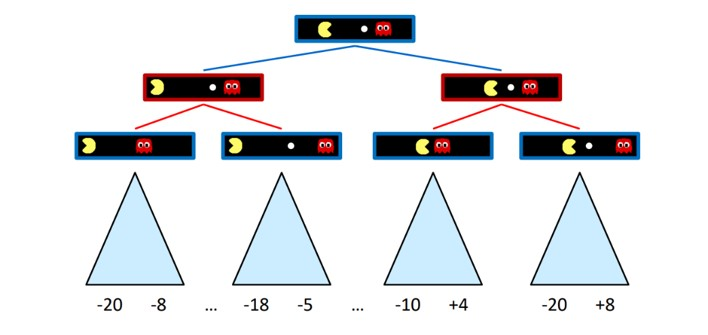
\includegraphics[width=0.8\linewidth]{images/adversarial02.jpg}
    \caption{Search Adversarial}
\end{figure}

این درخت با درخت Agent Single متفاوت است و نمیتوانیم مانند قبل بیشترین امتیاز هر فرزند را به گره بالای آن بدهیم چون رقیب ما میتواند راهی را انتخاب کند که ماکسیمم نباشد بلکه مینیمم باشد و سعی کند کمترین امتیاز را به شما بدهد.


\begin{figure}[h!]
    \centering
    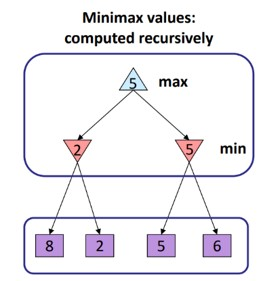
\includegraphics[width=0.4\linewidth]{images/minimax01.jpg}
    \caption{Minimax}
\end{figure}


\subsection{Minimax}
یکی از الگوریتم ها استفاده از minimax است که در حقیقت وقتی نوبت حریف است باید مینیمم امتیاز را برای گره قرار دهید ولی اگر نوبت شما باشد باید از فرصت استفاده کنید و بیشتری مقداری که میتوانید را برداشت کنید.

\begin{figure}[h!]
    \centering
    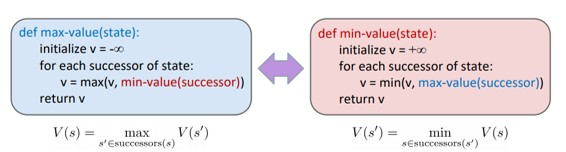
\includegraphics[width=0.8\linewidth]{images/minimax02.jpg}
    \caption{Code Minimax}
\end{figure}

همانطوری که مشاهده میکنید ما basecase ای نداریم و برای قابل پیاده سازی شدن باید یک حالت basecase برای این الگوریتم بازگشتیمان در نظر بگیریم که اکثرا بدلیل نمایی بودن رشد درخت قادر به جستوجوی کامل آن نیستیم و این کار امکان پذیر نیست که در آنجا به عنوان مثال می گوییم که تا 10000000 سطح پایین را بگردد و بعد دیگر ادامه ندهد.(Depth-limited)

\begin{figure}[h!]
    \centering
    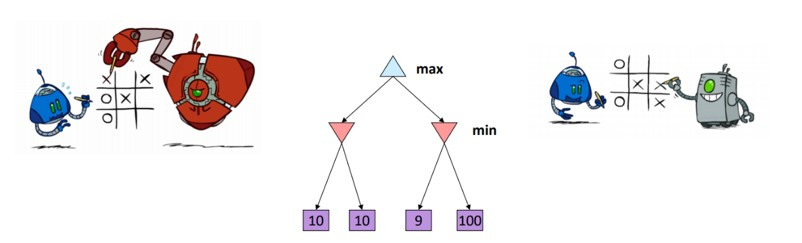
\includegraphics[width=0.8\linewidth]{images/minimax03.jpg}
    \caption{Minimax}
\end{figure}

اگر در مقابل یک حریف سرسخت و قوی بازی کنیم minimax نتیجه ی خوبی از بازی دریافت میکند ولی اگر رقیب ما ضعیف باشد agent به دلیل ترس از از دست دادن امتیاز ریسک نمی کند و این باعث میشود که از اشتباهات حریفش به خوبی استفاده نکند که دقیقا نقطه منفی این الگوریتم است.
کارآمدی این الگوریتم مانند dfs است. پیچیدگی زمانی این الگوریتم O(bn) است که b تعداد حالت یا factor branch است  و n هم عمق ما است. در مورد حافظه وضعیت بر خلاف زمانی بهتر است  و از O(bn) است. برای شطرنج factor branching 35 است و باید تا 100 سطح سرچ کنیم که امکان پذیر نیست. پس باید به دنبال راه حل دیگری باشیم.



\subsection{Pruning(Alpha-Beta) Minimax}

\begin{figure}[h!]
    \centering
    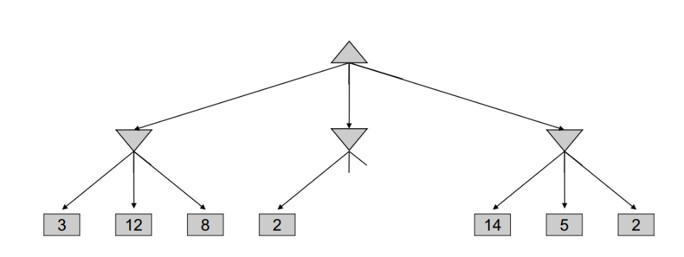
\includegraphics[width=0.8\linewidth]{images/pruning01.jpg}
    \caption{Pruning Minimax}
\end{figure}

یکی از راه هایی که به ما در بهینه‏ تر کردن الگوریتم کمک میکند pruning است به عنوان مثال درخت بالا را در نظر بگیرید در بین گرده های سمت چپ 3 کمتر است و به عنوان option best برای گره ریشه ی ما برگردانده میشود. ولی زمانی که گره میانی را بررسی میکنیم به عدد 2 برخورد میکنیم که از option best ما کمتر است. در حقیقت این بدین معنا است که عددی کوچکتر یا مساوی با 2 برگردانده خواهد شد که در هر صورت در بالا انتخاب نخواهد شد چون 3 از آن بزرگتر میباشد برای همین دیگر بقیه گره ها را بررسی نخواهیم کرد و همان 2 را باز میگردانیم.

\begin{figure}[h!]
    \centering
    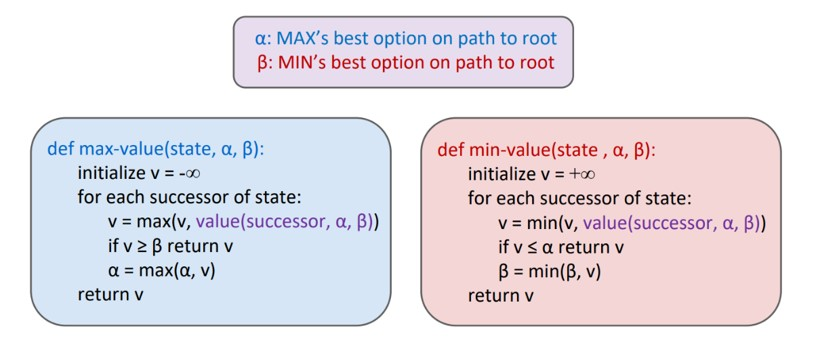
\includegraphics[width=0.8\linewidth]{images/pruning02.jpg}
    \caption{Code Pruning Minimax}
\end{figure}

همانطور که میبینید علاوه بر دادن وضعیت، آلفا و بتا نیز داده میشودند که نمادی از بیشترین و کمترین کاندیدا برای انتخاب شدن در مسیر رسیدن به root هستند.  همانطوری که ملاحظه میکنید زمانی که آلفا بزرگتر از گره‎ ای باشد که دارد بررسی میشود با بلعکس بلافاصله برگردانده میشود تا الگوریتم ما بهینه‎ تر باشد.
 نکته ای که باید به آن توجه داست این است که اگر child های یک گره به ترتیب و sort وشده باشند این بهینه بودن بیشتر خواهد شد. با این که پیچیدگی زمانی ما به O(b(n/2)) کاهش پیدا میکند. 
در این الگوریتم و در جواب نهایی که بر روی root نوشته خواهد شد تاثیری نخواهد داشت. این در حالی است که گره های میانی ممکن است دقیق نباشند.


\subsection{search limited Depth}
با وجود تلاشی که برای بهینه کردن minimax با عملیات pruning داشتیم هنوز امکان سرچ کامل را برای شطرنج نخواهیم داشت و مجبوریم از search limited Depth استفاده کنیم که همانطور که قبلا هم گفته شد بررسی و سرچ کردن گره ها تا سطح خاصی ادامه پیدا کند. منتهی مشکل این الگوریتم این است که دیگر بهینه بودن جواب را تضمین نخواهد کرد.

\subsection{function Evaluatoin}
function Evaluatoin چیزی شبیه به heuristic در a* است که مشخص میکند تا چه زمانی این سرچ ادامه پیدا کند. بعنوان مثال  function Evaluatoin  برای بازی شطرنج می تواند تعداد وزیر باشد. چون معمولا زمانی که وزیر بیرون خواهد رفت بازی برای حریف سخت تر خواهد شد. البته مشکل function Evaluatoin ها دقیقا همین است که همیشه عالی و کامل نیستند و شاید به درستی نتوانند موقعیت مناسب را پیدا کنند. در این جا هم یک Trade-off داریم که هر چقدر برای function Evaluatoin کمتر وقت بگذاریم عمیق تر میتوانیم برویم و هر چقدر بیشتر برای آن وقت بگذاریم function Evaluatoin ما دقیق تر خواهد شد. دقیقا مانند اتفاقی که در A* و برای Heuristic داشتیم.

\section{Search Expectimax}
همانطور که گفتیم اگر از الگوریتم minimax استفاده کنیم به دلیل آن که minimax خیلی محتاطانه رفتار می‎کند نمی تواند از اشتباهات رقیب به عنوان یک فرصت برای امتیاز بیشتر استفاده کند و آن را انتخاب نمیکند.
در روش جستجوی expectimax ما درخت جدیدی را در نظر میگیریم که به جای مینیمم بچه های آن گره میانگین را در آن قرار میدهد که به شکل زیر است.


\begin{figure}[h!]
    \centering
    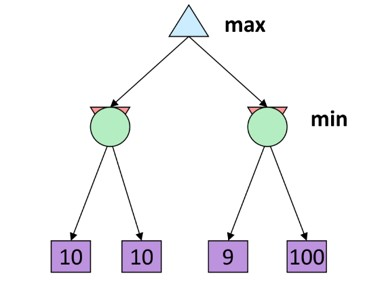
\includegraphics[width=0.4\linewidth]{images/expectimax01.jpg}
    \caption{Expectimax}
\end{figure}

به عنوان مثال در شکلی که ملاحظه می کنید گره سمت چپ برابر 10 و گره سمت راست برابر میانگین 9 و 100 خواهد شد که 54.5 است. و بنابراین گره max ما مسیر سمت راست را انتخاب خواهد کرد.

\begin{figure}[h!]
    \centering
    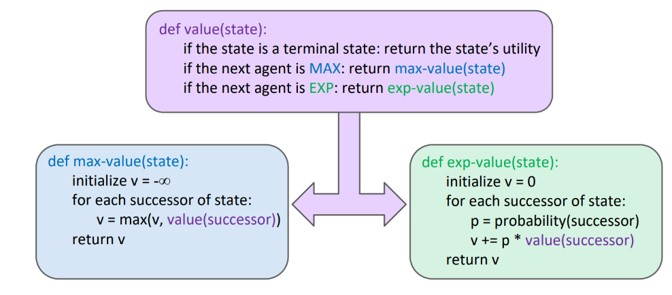
\includegraphics[width=0.8\linewidth]{images/expectimax02.jpg}
    \caption{Code Expectimax}
\end{figure}

سودوکد الگوربتم نیز خیلی شبیه به minimax است فقط با این تفاوت که بجای min گرفتن average گرفتن داریم (محاسبه احتمال).  نکته ای که وجود دارد ما در این جا عملیات pruning نداریم و برای محاسبه میانگین لازم است که تمام بچه های یک گره دیده شوند و محاسبه را برای ان‎ها انجام دهیم پس روش ما Depth-Limited است یعنی به علت محدودیت زمانی تا عمق خاصی این عملیات را می توانیم که انجام بدهیم و بعد از رسیدن به عمقی خاص باید عملیات جستوجو را متوقف نماییم.
دلیلی که باعث می‎شود ما از این روش استفاده کنیم مشخص نبودن نتیجه در صورت انتخاب یک action  هست که می‎تواند دلایل خاصی داشته باشد.

\begin{itemize}
    \item
طراحی بازی به گونه ای است که deterministic نباشد و متغییری مانند تاس داشته باشیم.
    \item
حرکت طرف مقابل قابل پیشبینی نباشد و بخواهیم جوری بازی را مدل کنیم که از اشتباهات رقیبمان نیز استفاده کنیم. مانند ghost ها در بازی  pacman.
    \item
به دلیل fail شدن action ای که انتخاب کردیم. مثلا یک روبات در حرکت کردن به سمت شمال ممکن است موفق نباشد و باید احتمالی را در نظر بگیریم. (برای مواقعی که امکان درست اجرا نشدن action ها وجود دارد.)
\end{itemize}

در این الگوریتم باید به نکته ای توجه کنیم و آن نتیجه ی این بازی است. نتیجه بازی هیچ وقت برابر 54 و نیم نمی شود نتیجه همیشه یا 9 است یا 100 ولی این عدد بیانگر این موضوع است که اگر به دفعات این بازی را انجام دهیم امتیازی که از آن می گیریم برابر 54 و نیم خواهد بود. در ضمن در MDP بیشتر در مورد اینگونه مواردی که نتیجه مشخص نیست صحبت خواهد شد.

اگر شرایطی داشته باشیم که رقیب ما در 80 درصد مواقع یک minimax به عمق 2 را اجرا نماید و در غیر اینصورت بطور رندوم حرکت کند بهترین کار این است که ما نیز در 20 درصد مواقع expectimax را اجرا نماییم تا از فرصت رندوم بودن و غیر هوشمند بودن تصمیمات رقیبمان استفاده کنیم. همانطور که می‎بینید می توانیم یکسری inform-probability نیز داشته باشیم و ساختار درخت ما به‎گونه ای mix شده و ترکیبی باشد و هدف از این مثال نیز همین بود.

\section{Optimism And Pessimism}

در اینجا می خواهیم در مورد خوشبین بودن یا محتاط بودن بیش از اندازه صحبت کنیم. اگر بسیار خوش بین باشید در بعضی مواقع به مواردی بر‎خواهید خورد که به دلیل خوش بین بودن شما به مسئله، امتیازی را از دست خواهید داد. برعکس آن نیز درست است اگر خیلی محتاط باشید ممکن است از خیلی از فرصت هایی که به سود شما است استفاده نکنید.

\begin{figure}[h!]
    \centering
    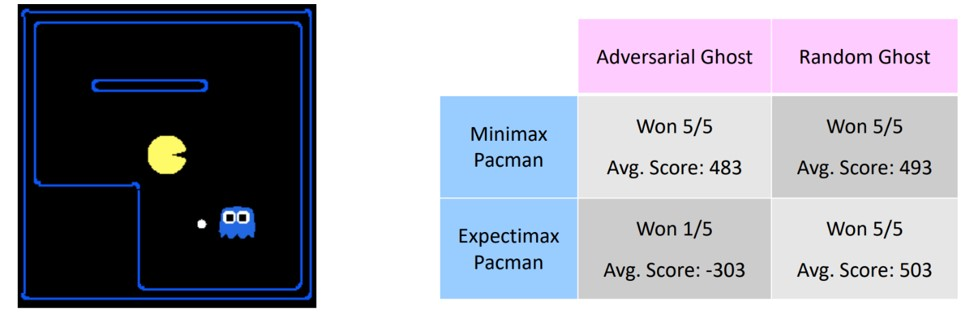
\includegraphics[width=0.8\linewidth]{images/PacmaninOptimismAndPessimism.jpg}
    \caption{Pacman in Optimism And Pessimism}
\end{figure}


در اینجا ما حالت های مختلف بازی pacman را در نظر گرفته ایم. همانطور که می بینید وقتی بصورت minimax بازی کنیم چه در مقابل یک ghost رندوم و چه در مقابل یک ghost باهوش باشیم بازی را مبیریم. اما این نکته حائز اهمیت است که اگر زمانی که ghost رندوم است از الگوریتم expectimax استفاده می‎کردیم امتیاز بیشتری را میتوانستیم کسب کنیم. اما expectimax نیز در مقابل یک ghost هوشمند خیلی خوش بین خواهد بود و امتیاز از دست میدهد.

\section{Types Game Other}

\subsection{types Layer Mix}

\begin{figure}[h!]
    \centering
    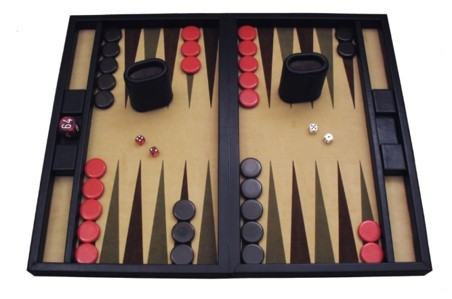
\includegraphics[width=0.6\linewidth]{images/backgammon.jpg}
    \caption{Backgammon}
\end{figure}

ما بازی هایی را با درخت minimax و expectimax بیان کردیم و بازی های دیگری نیز وجود دارند که درخت های آن ها به شکل های دیگری هستند. در حقیقت همه ی آن‎ها همین گره های  min ،  max یا average را دارند ولی بصورت ترکیبی هستند. که به آن ها types Layer Mix  می گویند. به عنوان مثال در بازی تخته نرد یک متغییر به نام تاس داریم که باعث می‎شود شکل درخت ما بصورت زیر بشود.

\begin{figure}[h!]
    \centering
    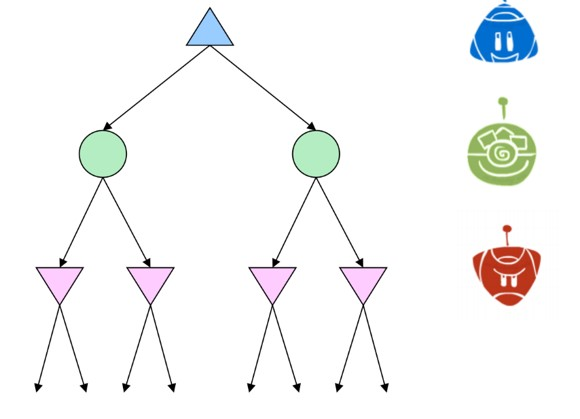
\includegraphics[width=0.6\linewidth]{images/backgammonTree.jpg}
    \caption{Tree Backgammon}
\end{figure}

اگر بخواهیم محاسباتی برای درخت تخته نرد تا سطح دوم داشته باشیم:

در هر حرکت ما به طور میانگین 20 حرکت میتوانیم انجام دهیم و همچنین 21 امکان برای تاس وجود دارد چون دو تاس داریم و تعداد حالات غیر تکراری آن برابر 21 خواهد شد. حال با توجه به این که در ابتدا احتمالی برای تاس نداریم (چون تاس ها ریخته شده اند و مقادیر آن‎ها مشخص شده است) محاسبه سطح دوم درخت به شکل زیر است:

\begin{equation}
20 \times (21 \times 20)^3 = 1.2 \times 10^9
\end{equation}

که در حقیقت عبارت زیر بوده است ولی چون تاس ها در لحظه تصمیم گیری ریخته شده اند یک تقسیم بر 21 دارد.
\begin{equation}
(21 \times 20)^4
\end{equation}


\subsection{types Multi-agent}
در بعضی از بازی ها ما چندین بازیکن داریم و پیشبینی را باید به تعداد بازیکن ها و با توجه به امتیازهایی که میگیرند انجام دهیم.

\begin{figure}[h!]
    \centering
    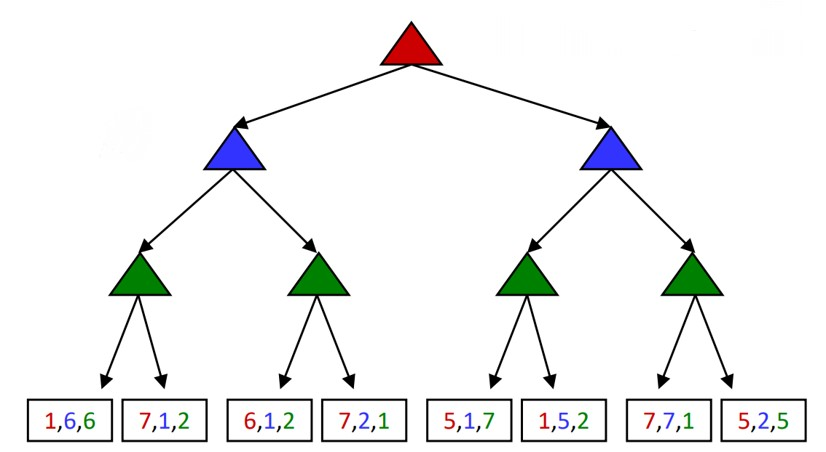
\includegraphics[width=0.8\linewidth]{images/multiagentTree.jpg}
    \caption{Tree Multi-agent}
\end{figure}

به عنوان مثال ما در اینجا 3 بازیکن داریم و باید از پایین شروع کنیم و درگره های سبز رنگ مواردی را بر می داریم که برای سبز بیشترین سودمندی (utility) را داشته باشد. در ادامه همین روند را پیش می گیریم و از بین آن‎هایی که انتخاب شدند آن‎هایی که برای آبی بیشترین سودمندی را داشته باشند درون گره مقدار دهی می شوند در نتیجه گره قرمز رنگ از بین (1,6,6) و (5,2,5) آن را که سودمندی بیشتری دارد انتخاب میکند. (5,2,5)

\section{Utilities}
در این جا کمی می‎خواهیم در مورد خود سودمندی ها صحبت کنیم.

\begin{figure}[h!]
    \centering
    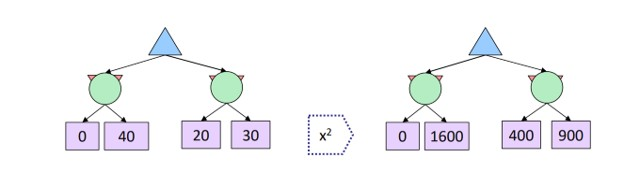
\includegraphics[width=0.8\linewidth]{images/utilities01.jpg}
    \caption{Difference Utilities}
\end{figure}

نکت ‎ای که وجود دارد خود امتیازها و سودمندی ها حتی میتواند روی الگوریتم و شیوه تصمیم گیری ما تاثیر بگذارند. به عنوان مثال درخت رو‎ به رو را در نظر بگیرید که در آن ما ارزش هر گره را مجذوز کرده ایم. برای minimax ما دقیقا همان نتیجه قبلی را داریم ولی برای expectimax نتیجه‎ی متفاوتی خواهیم داشت که این نتیجه به ما نشان می‎دهد حتی مقادیر سودمندی می‎تواند تصمیمات ما را تغییر دهد.

\subsection{Preferences Rational}
در اینجا ما روابطی داریم که باید برای سناریو و شروط ما (Constraints) برقرار باشند. به عنوان مثال اگر A سودمند تر از B باشید و B هم سودمند تر از C باشد حتما باید A از C سودمند تر باشد. که به شکل زیر نمایش میدهیم. حال اگر این رابطه برقرار نباشد چه اتفاقی می‎افتد.

\begin{figure}[h!]
    \centering
    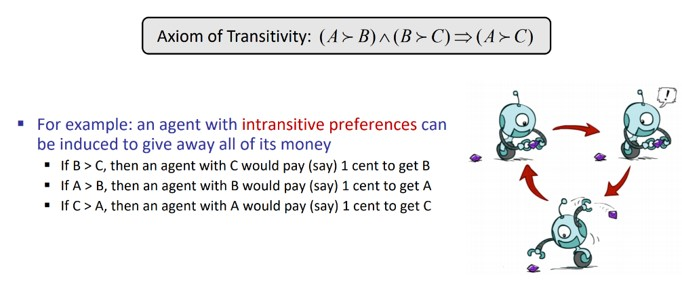
\includegraphics[width=0.8\linewidth]{images/transivity.jpg}
    \caption{Transitivity}
\end{figure}


اتفاقی که می افتد این است که Agent ما قادر به تصمیم گیری نخواهد بود و پی در پی تصمیم خود را به دلیل این که دیگری تصمیم بهتری است عوض می کند. مانند نمونه بالا روابط و شروطی وجود دارند که باید برقرار باشند و بعد از داشتن این موارد سناریوی ما اصطلاحا confirmed rationality میشود.

\begin{figure}[h!]
    \centering
    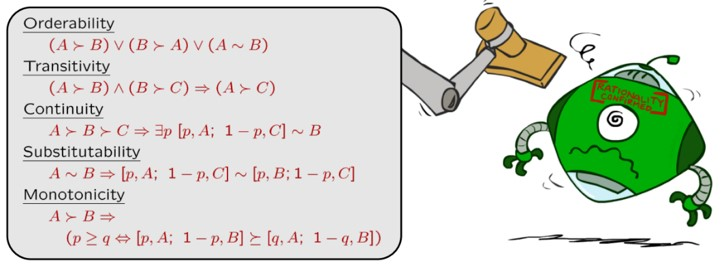
\includegraphics[width=0.8\linewidth]{images/rationality.jpg}
    \caption{Constraints Rational}
\end{figure}

\subsection{Utilities Human}
در زندگی روزمره، انسان ها تصمیماتی میگیرند که در آن‎ها احتمالات و سودمندی را سنجش می‎نمایند ولی در مواردی مانند لاتری و درمورد پول کمی این موضوع متفاوت است. ارزش پول نسبی است برای کسی که پولی ندارد یک میلیون دلار خیلی زیاد است ولی برای کسی که میلیاردر است شاید این مقدار سودمندی ای نداشته باشد و همینطور برعکس کسی که مقدار زیادی بدهکار باشد آمدن مقداری بدهی بروی آن برایش کم اهمیت تر است. با وجود این صحبت ها به همچین نموداری خواهیم رسید.

\begin{figure}[h!]
    \centering
    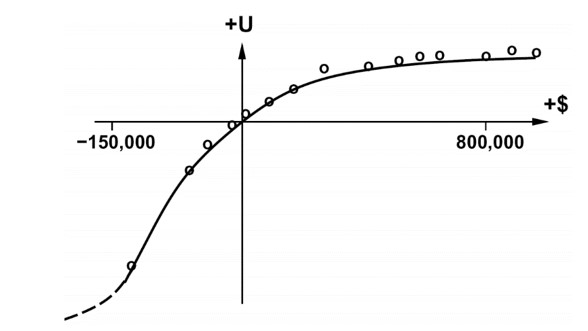
\includegraphics[width=0.6\linewidth]{images/moneyUtility.jpg}
    \caption{Chart Utility Money}
\end{figure}


حال می خواهیم آزمایشی انجام دهیم کدام یک از لاتری‎های زیر را انتخاب میکنید.

\begin{figure}[h!]
    \centering
    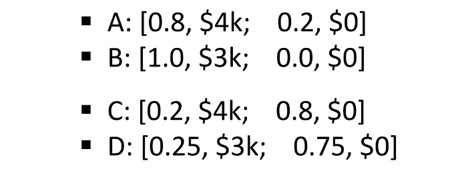
\includegraphics[width=0.6\linewidth]{images/lottery01.jpg}
    \caption{lotteries}
\end{figure}

اکثر آدم ها لاتری A و  C را انتخاب میکنند و این نشان دهنده این است که همیشه آدم ها منطقی و ریاضیاتی فکر نمیکند. برای مورد  C این تصمیم منطقی است ولی برای مورد اول نه:\

\begin{figure}[h!]
    \centering
    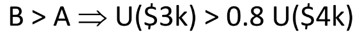
\includegraphics[width=0.6\linewidth]{images/lottery02.jpg}
    \caption{Utility Calculate}
\end{figure}

همانطوری که احساس می کنید با این که سودمندی و یا utility بیشتری دارد اما بیشتر آدم ها آن را انتخاب می کنند که یکی از دلایل آن می تواند این باشد که اعصاب خوردی آن 20 درصد خیلی تاثیر منفی روی انسان ها داشته باشد. البته این که در یک لاتری داریم شرکت میکنیم با دنباله ای از لاتری ها باشد ممکن است در تصمیم گیری بعضی افراد تاثیر گذار باشد. چون اگر 100 لاتری بدین شکل داشته‎ باشیم بعضی از انسان ها میانگین سودهایشان از لاتری را محاسبه میکنند و ممکن است مورد B را انتخاب کنند.